\documentclass{article}

% Định dạng chuẩn NeurIPS 2024
\usepackage[preprint]{neurips_2024}

% Hỗ trợ tiếng Việt với mã hóa T5 và bảng mã UTF-8
\usepackage[utf8]{inputenc}
\usepackage[vietnamese]{babel}
\usepackage[T5]{fontenc}

\usepackage[numbers]{natbib}
\usepackage{hyperref}
\usepackage{url}
\usepackage{booktabs}
\usepackage{amsfonts}
\usepackage{amsmath}
\usepackage{amssymb}
\usepackage{nicefrac}
\usepackage{microtype}
\usepackage{graphicx}
\usepackage{xcolor}
\usepackage{subcaption}
\usepackage{multirow}

\hypersetup{
    colorlinks=true,
    linkcolor=blue!75!black,
    citecolor=green!50!black,
    urlcolor=blue!80!black
}

\title{Đánh giá Benchmark sinh dữ liệu bất thường dạng bảng trong công nghiệp:\\Khai thác mô hình học sâu học trên dữ liệu chuẩn\\dưới điều kiện mất cân bằng cực đoan}

\author{%
  \textbf{Đào Thế Việt} \\
  Email: \texttt{daothevietnb123@gmail.com} \\
  \And
  \textbf{Đặng Cao Cường} \\
  Email: \texttt{caocuong7a2@gmail.com} \\
  \AND
  \normalfont
  Bộ môn Trí tuệ Nhân tạo (Department of Artificial Intelligence) \\
  Trường Đại học FPT (FPT University) \\
  Môn học: DAP391m \\
}

\begin{document}

\maketitle

\begin{abstract}
Trong các hệ thống điều khiển công nghiệp và bài toán bảo trì dự đoán (Predictive Maintenance), việc thu thập dữ liệu sự cố là cực kỳ khó khăn, tốn kém chi phí và tiềm ẩn nguy cơ phá hủy máy móc nghiêm trọng, dẫn đến tình trạng mất cân bằng dữ liệu cực đoan. Các mô hình phân loại có giám sát truyền thống hoàn toàn sụp đổ trong điều kiện vận hành an toàn không lỗi (Zero-Defect regime), trong khi các phương pháp học không giám sát kinh điển gặp khó khăn khi phân định đường biên lỗi trong không gian cảm biến đa chiều phi tuyến. Trong nghiên cứu này, chúng tôi phát triển một hệ thống theo kiến trúc module hóa (\emph{Everything is a Plugin}), chuyên biệt cho việc tổng hợp dữ liệu bất thường dạng bảng sát biên bằng cách huấn luyện 100\% trên dữ liệu vận hành bình thường. Chúng tôi triển khai và đối chứng ba mô hình sinh tiên tiến: \textbf{TVAE}, \textbf{Fence GAN}, và \textbf{TabDDPM}. Toàn bộ hệ thống được thẩm định trên hai bộ dữ liệu thực tế: Trạm tuần hoàn nước SKAB Valve1 và Dây chuyền phay tiện CNC AI4I 2020 thông qua hệ thống đo đạc 3 tầng: tính chân thực biên (Fidelity), bảo toàn ma trận tương quan vật lý (Correlation), và hiệu năng phân loại thực chiến hạ nguồn (Utility TSTR). Kết quả cho thấy dữ liệu bất thường nhân tạo giúp bộ phân loại tiệm cận và vượt qua mức trần có giám sát ($F_1 \approx 0.658$ trên SKAB và tăng vượt bậc từ $0.222$ lên $0.317$ trên AI4I so với Isolation Forest), chứng minh tính khả thi vượt trội của phương pháp tổng hợp dị biệt biên. Toàn bộ mã nguồn và pipeline thực nghiệm được công khai tại \url{https://github.com/TeamToTe/dap-viet-cuong}.
\end{abstract}

%%%%%%%%%%%%%%%%%%%%%%%%%%%%%%%%%%%%%%%%%%%%%%%%%%%%%%%%%%%%%%%%%%%%%%%%%%%%%%%
\section{Giới thiệu \& Các Bộ Dữ liệu Công nghiệp Chuẩn}
\label{sec:intro_data}
%%%%%%%%%%%%%%%%%%%%%%%%%%%%%%%%%%%%%%%%%%%%%%%%%%%%%%%%%%%%%%%%%%%%%%%%%%%%%%%

Trong các hệ sinh thái sản xuất thông minh Công nghiệp 4.0 (Smart Manufacturing), hệ thống giám sát và thu thập dữ liệu tự động (SCADA) đo lường liên tục hàng loạt cảm biến vật lý. Trong thực tế, máy móc được thiết kế và bảo dưỡng tối ưu nhằm duy trì trạng thái vận hành ổn định trên 99\% thời gian. Việc cố ý gây sự cố hoặc phá hủy máy để thu thập mẫu bất thường là điều hoàn toàn bị cấm kỵ vì gây thiệt hại hàng triệu đô la và đình trệ dây chuyền sản xuất~\citep{katser2021skab, matzka2020explainable}. Đây chính là bài toán \emph{Mất cân bằng dữ liệu cực đoan} (Extreme Class Imbalance).

Để giải quyết triệt để rào cản này, chúng tôi tiếp cận theo hướng \emph{One-Class Deep Generative Formulation}: Mô hình sinh chỉ được phép học trên tập dữ liệu vận hành an toàn bình thường (100\% Normal samples $\mathcal{D}_{\text{train}}^{\text{normal}}$), sau đó kích hoạt các cơ chế nhiễu loạn có kiểm soát để tự động sản sinh các mẫu lỗi nhân tạo bám sát đường viền dung sai cơ lý. Chúng tôi kiểm chứng phương pháp luận trên hai trạm thực nghiệm công nghiệp:

\paragraph{Bộ dữ liệu 1: SKAB Valve1 (Skoltech Anomaly Benchmark).} Được xây dựng bởi Phòng thí nghiệm Hệ thống Không gian Mạng thuộc Viện Skolkovo (Nga)~\citep{katser2021skab}, SKAB mô phỏng trạm tuần hoàn chất lỏng công nghiệp khép kín gồm bơm ly tâm, van tiết lưu Valve1, đường ống dẫn thủy lực và mạng lưới 8 cảm biến đo liên tục với tần số 1 Hz (Bảng~\ref{tab:datasets}). Chúng tôi áp dụng chiến lược phân chia \emph{Zero-Defect split}: 9 lần chạy đầu tiên (chỉ chứa 100\% mẫu bình thường, nhãn lỗi $y=0$) được cô lập làm tập huấn luyện Train; 7 lần chạy độc lập còn lại chứa các sự cố kẹt van và biến thiên dòng thủy lực thực tế được giữ làm tập kiểm thử Test.

\paragraph{Bộ dữ liệu 2: AI4I 2020 Predictive Maintenance.} Được đóng góp bởi Matzka~\citep{matzka2020explainable} trên kho lưu trữ UCI Machine Learning Repository, bộ dữ liệu phản ánh quy trình gia công cơ khí phay tiện CNC với đúng 10,000 bản ghi dữ liệu bảng. Tỷ lệ lỗi trong thực tế chỉ có 339 mẫu (chiếm $3.39\%$). Tập dữ liệu theo dõi 5 biến cảm biến nhiệt động học và động lực học (Nhiệt độ không khí, Nhiệt độ gia công, Tốc độ quay trục chính, Mô-men xoắn, và Độ mòn dao) tương ứng với 5 hình thái hư hỏng cụ thể: Mòn dao (TWF), Tản nhiệt kém (HDF), Công suất quá tải (PWF), Quá tải lực căng (OSF), và Sự cố ngẫu nhiên (RNF).

\begin{table}[t]
\centering
\caption{Đặc tả kỹ thuật và ý nghĩa vật lý công nghiệp của các biến cảm biến trong benchmark.}
\label{tab:datasets}
\resizebox{\textwidth}{!}{%
\begin{tabular}{@{}llllp{7.0cm}@{}}
\toprule
\textbf{Bộ dữ liệu} & \textbf{Biến cảm biến} & \textbf{Đơn vị} & \textbf{Kiểu dữ liệu} & \textbf{Ý nghĩa vật lý công nghiệp thực tế} \\ \midrule
\multirow{4}{*}{\textbf{SKAB Valve1}} & Accelerometer1RMS / 2RMS & $g$ ($\text{m/s}^2$) & Liên tục & Độ rung động hiệu dụng trục chính trên thân bơm và chân đế \\
 & Pressure & $\text{bar}$ & Liên tục & Áp suất thủy lực dòng nước trước/sau cụm van tiết lưu \\
 & Volume Flow RateRMS & $\text{m}^3/\text{h}$ & Liên tục & Vận tốc lưu lượng thể tích chất lỏng tuần hoàn trong hệ thống \\
 & Current / Voltage & $\text{A} / \text{V}$ & Liên tục & Dòng điện tiêu thụ động cơ bơm và điện áp nguồn cung cấp \\ \midrule
\multirow{3}{*}{\textbf{AI4I 2020}} & Air / Process Temp & $\text{K}$ & Liên tục & Nhiệt độ phòng máy và nhiệt độ ma sát tại mũi dao cắt \\
 & Rotational Speed & $\text{rpm}$ & Liên tục & Tốc độ quay trục chính (Spindle) gắn dao phay \\
 & Torque / Tool Wear & $\text{Nm} / \text{phút}$ & Liên tục & Mô-men xoắn động cơ kéo và thời gian hao mòn mũi dao cụ \\ \bottomrule
\end{tabular}%
}
\end{table}

%%%%%%%%%%%%%%%%%%%%%%%%%%%%%%%%%%%%%%%%%%%%%%%%%%%%%%%%%%%%%%%%%%%%%%%%%%%%%%%
\section{Kiến trúc Hệ thống \& Quy trình Thực nghiệm}
\label{sec:pipeline}
%%%%%%%%%%%%%%%%%%%%%%%%%%%%%%%%%%%%%%%%%%%%%%%%%%%%%%%%%%%%%%%%%%%%%%%%%%%%%%%

Tính tái lập (reproducibility) và khả năng mở rộng (extensibility) là tiêu chí sống còn khi xây dựng hệ thống thử nghiệm AI công nghiệp. Thay vì viết code nguyên khối hay dồn vào Jupyter Notebook rất khó bảo trì, hệ thống được thiết kế theo triết lý \textbf{``Everything is a Plugin''}. Toàn bộ mã nguồn, cấu hình và kịch bản thực nghiệm được cung cấp công khai tại \url{https://github.com/TeamToTe/dap-viet-cuong}.

\begin{figure}[htbp]
\centering
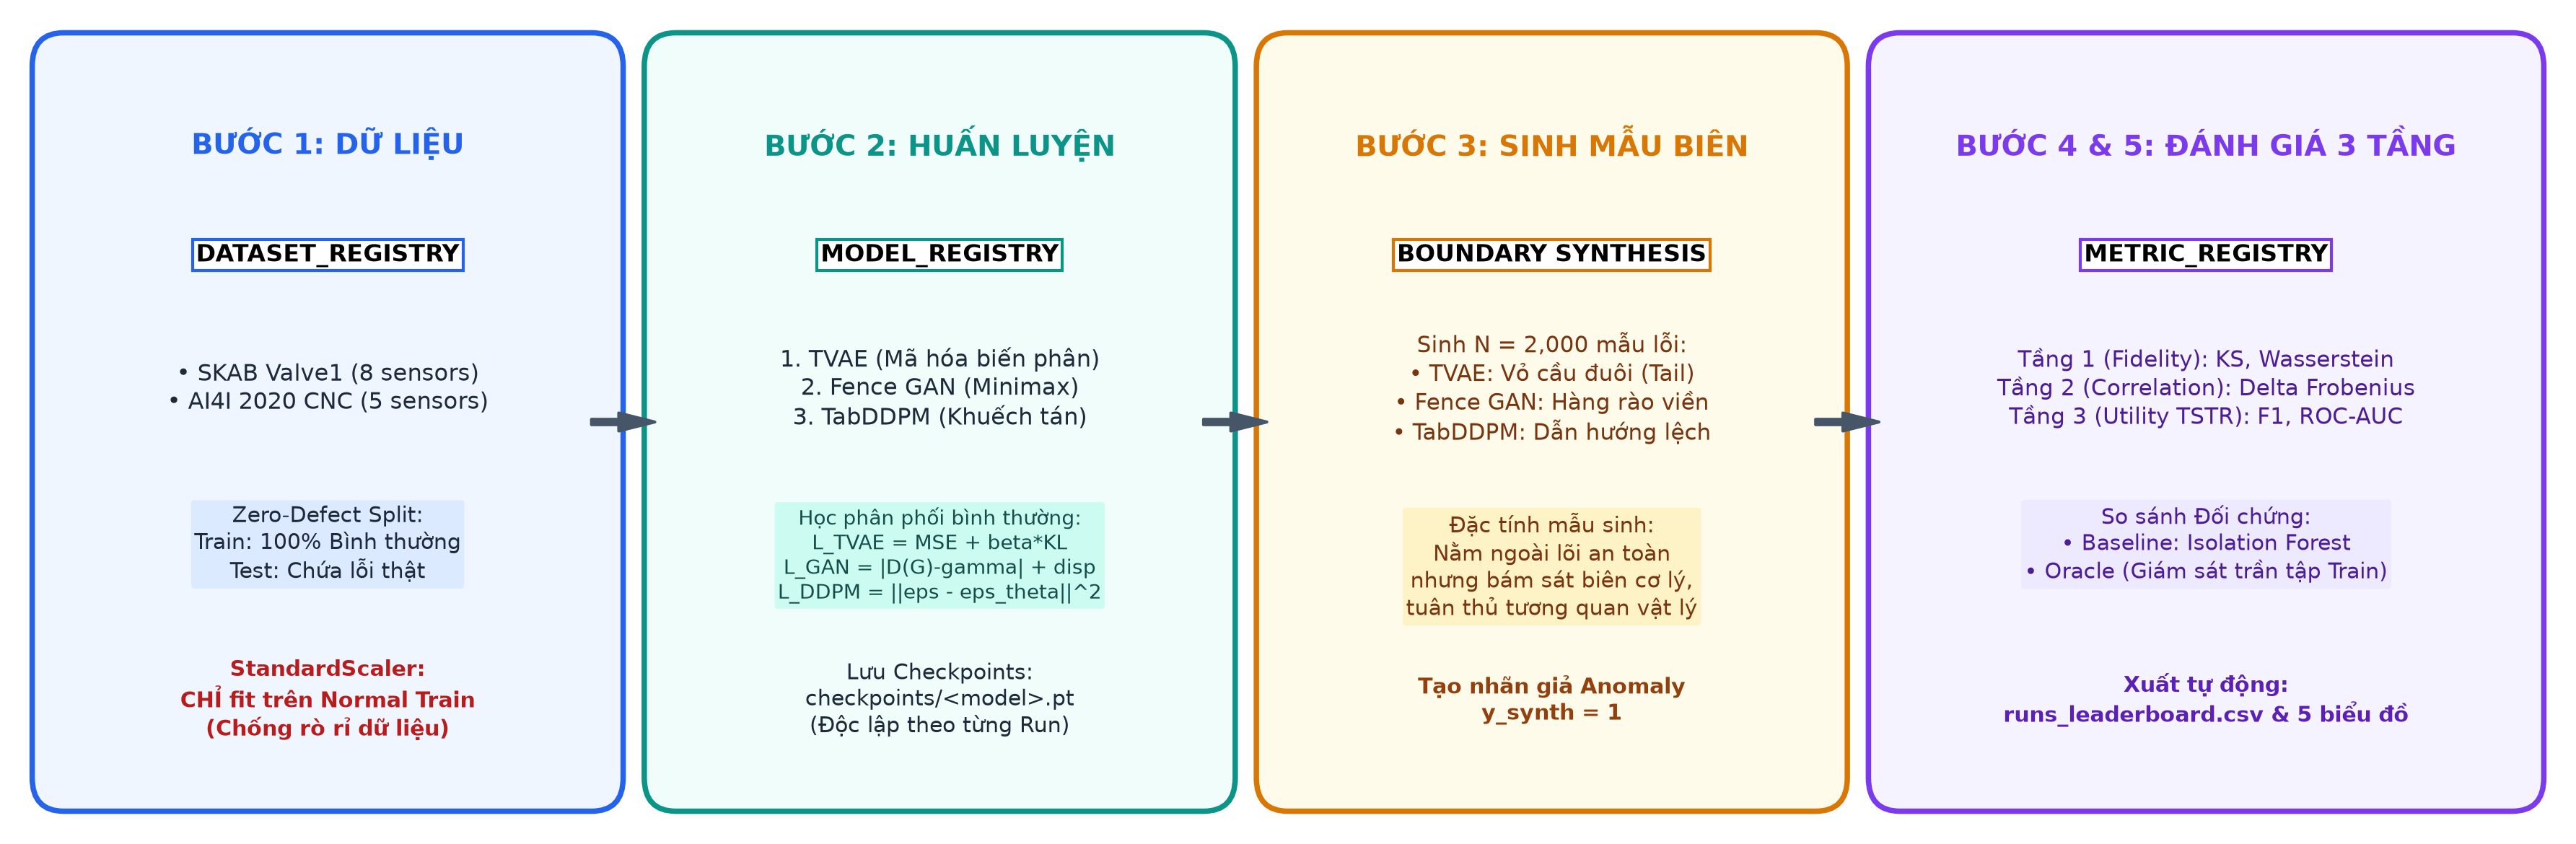
\includegraphics[width=\linewidth]{figures/pipeline_architecture.png}
\caption{Quy trình luồng thực thi đường ống thực nghiệm End-to-End 5 bước dựa trên kiến trúc Registry Pattern. Toàn bộ quá trình chuẩn hóa được cách ly triệt để nhằm chống rò rỉ dữ liệu (Data Leakage), kết hợp sinh mẫu dị biệt biên và đánh giá đa tầng tự động.}
\label{fig:pipeline}
\end{figure}

\subsection{Mô hình Plugin Registry Pattern}
Hệ sinh thái mã nguồn tách rời hoàn toàn giao diện trừu tượng (Abstract Base Classes) và các thực thi cụ thể thông qua bộ đăng ký tập trung:
\begin{itemize}
    \item \texttt{DATASET\_REGISTRY}: Kế thừa \texttt{BaseDataset}, chuẩn hóa dữ liệu đầu ra \texttt{TabularDataResult} và metadata vật lý. Mở rộng bộ dữ liệu mới chỉ cần một decorator \texttt{@register\_dataset}.
    \item \texttt{MODEL\_REGISTRY}: Kế thừa \texttt{BaseGenerativeModel}, chuẩn hóa giao thức huấn luyện \texttt{fit(X\_train)} và giao thức sinh dị biệt biên \texttt{sample(n\_samples)}.
    \item \texttt{METRIC\_REGISTRY}: Tách độc lập các bộ đánh giá toán học và tiện ích phân loại hạ nguồn.
\end{itemize}

\subsection{Luồng thực thi End-to-End 5 bước}
Quy trình thực nghiệm vận hành tự động qua 5 bước liên hoàn (Hình~\ref{fig:pipeline}):
\begin{enumerate}
    \item \textbf{Nạp dữ liệu \& Tiền xử lý chống rò rỉ (Leak-Free Preprocessing):} Dữ liệu được nạp tự động. Để bảo đảm tính khách quan khoa học, bộ chuẩn hóa \texttt{StandardScaler} \emph{chỉ được fit trên tập Normal Train} $\mathcal{D}_{\text{train}}^{\text{normal}}$, sau đó áp dụng phép biến đổi \texttt{transform} sang tập Test nhằm tránh rò rỉ phân phối (Data Leakage).
    \item \textbf{Huấn luyện Mô hình sinh:} Huấn luyện TVAE, Fence GAN, và TabDDPM trên các tọa độ cảm biến đã chuẩn hóa. Trọng số tối ưu (\texttt{.pt}) và nhật ký hàm mất mát được lưu trữ cách ly theo từng phiên thử nghiệm (\texttt{experiments/runs/<run\_name>/}).
    \item \textbf{Sinh mẫu dị biệt biên có kiểm soát:} Mỗi mô hình tự động sản sinh $N=2,000$ mẫu bất thường nhân tạo bám sát đường bao ngoài của phân phối an toàn.
    \item \textbf{Đánh giá Đa tầng 3 cấp độ (3-Tier Evaluation):} Kiểm tra độ tương đồng phân phối 1 chiều (Fidelity), đo lường sai lệch ma trận tương quan đa chiều (Correlation), và kiểm định độ hữu dụng phân loại hạ nguồn TSTR (Downstream Utility).
    \item \textbf{Kết xuất Báo cáo \& Bảng tổng hợp đối chứng:} Tự động tổng hợp kết quả vào file \texttt{runs\_leaderboard.csv} và xuất đồng loạt các biểu đồ khoa học độ phân giải cao vào thư mục \texttt{figure/}.
\end{enumerate}

%%%%%%%%%%%%%%%%%%%%%%%%%%%%%%%%%%%%%%%%%%%%%%%%%%%%%%%%%%%%%%%%%%%%%%%%%%%%%%%
\section{Phương pháp sinh dữ liệu bất thường bằng mô hình học sâu}
\label{sec:models}
%%%%%%%%%%%%%%%%%%%%%%%%%%%%%%%%%%%%%%%%%%%%%%%%%%%%%%%%%%%%%%%%%%%%%%%%%%%%%%%

Khác với các mô hình sinh thông thường tập trung học để tái tạo lại vùng lõi phân phối $p_{\text{data}}(x)$, mục tiêu của bài toán này là \emph{sinh mẫu dị biệt có kiểm soát}: tạo ra các mẫu nằm ngoài miền vận hành an toàn nhưng không văng vào các tọa độ phi vật lý. Chúng tôi nghiên cứu 3 mô hình đại diện với kiến trúc và cơ chế sinh riêng biệt.

\subsection{Tabular Variational Autoencoder (TVAE)}
TVAE~\citep{xu2019modeling} ánh xạ vector cảm biến vật lý $x \in \mathbb{R}^D$ vào không gian tiềm ẩn đa biến $z \in \mathbb{R}^d$ ($d < D$). Bộ mã hóa Encoder xấp xỉ phân phối hậu nghiệm $q_\phi(z|x) = \mathcal{N}(\mu_\phi(x), \Sigma_\phi(x))$, trong khi Decoder $p_\theta(x|z)$ tái tạo lại vector ban đầu thông qua hàm mất mát ELBO:
\begin{equation}
\label{eq:tvae_loss}
\mathcal{L}_{\text{TVAE}}(\theta, \phi) = \mathbb{E}_{q_\phi(z|x)} \left[ \| x - \hat{x} \|_2^2 \right] + \beta \cdot D_{\text{KL}}\left( q_\phi(z|x) \,\|\, \mathcal{N}(0, I) \right)
\end{equation}
trong đó trọng số $\beta = 0.05$ giúp cân bằng giữa độ chính xác tái tạo và độ trơn của không gian ẩn. Kiến trúc mạng chi tiết được mô tả ở Hình~\ref{fig:tvae_arch}a.

\begin{figure}[htbp]
\centering
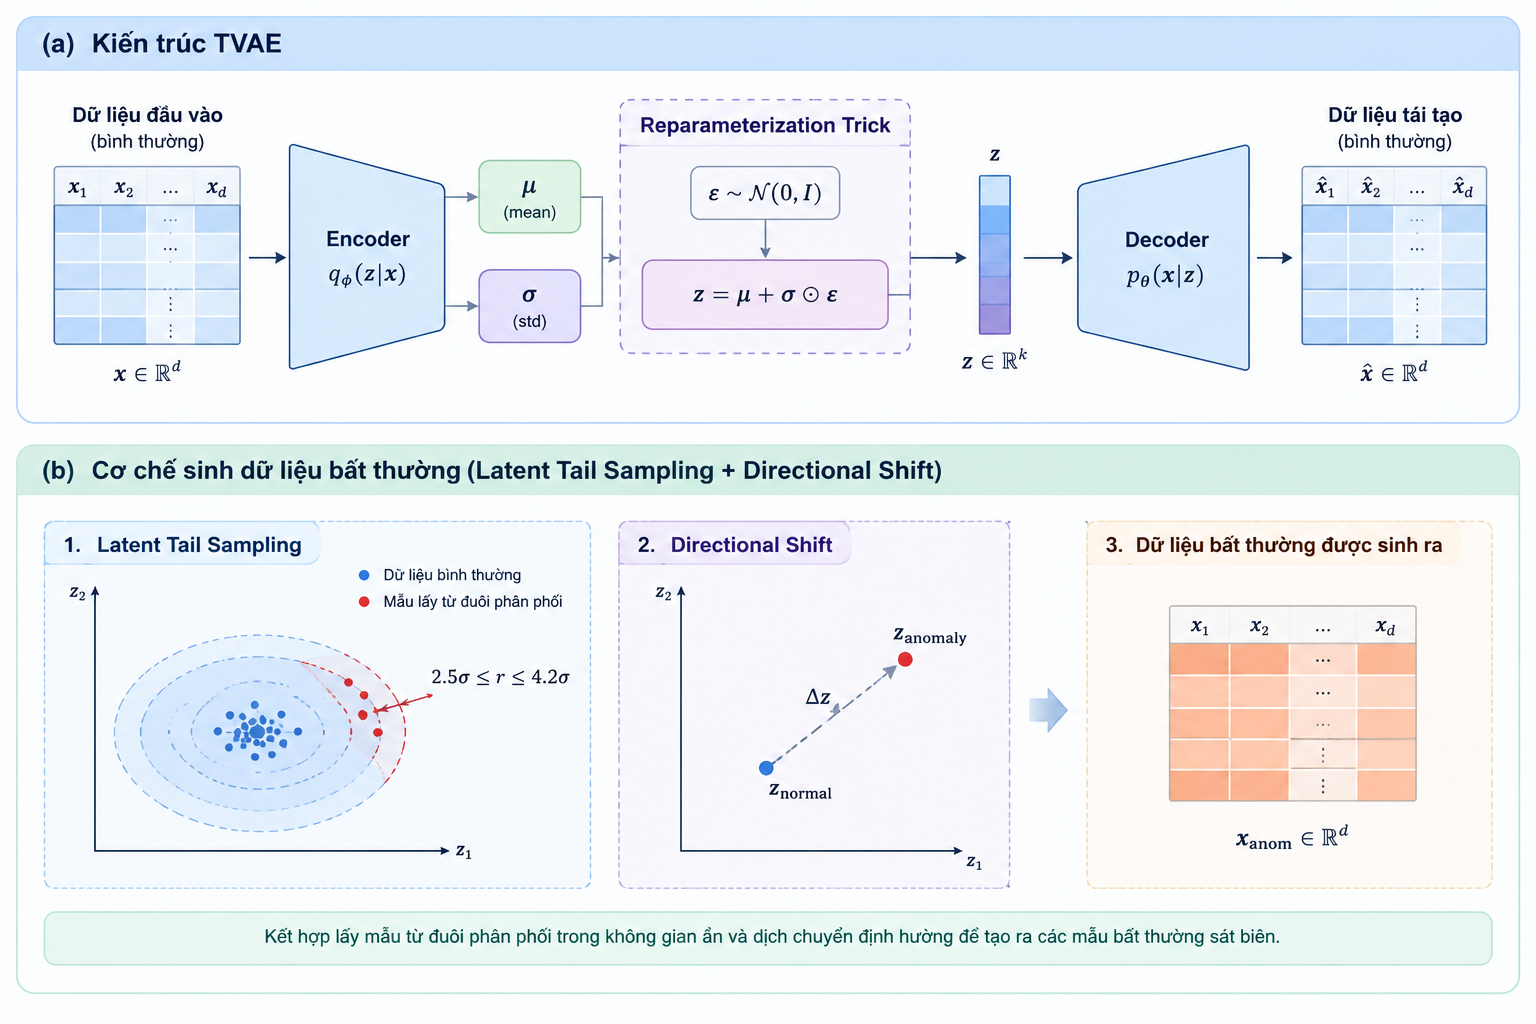
\includegraphics[width=0.85\linewidth]{figures/tvae.png}
\caption{Kiến trúc mạng Tabular VAE và cơ chế sinh dị biệt. \textbf{(a)} Cấu trúc Encoder, Reparameterization Trick và Decoder. \textbf{(b)} Cơ chế lấy mẫu ngoài vỏ cầu đuôi phân phối (Latent Tail Sampling $2.5\sigma \leq r \leq 4.2\sigma$) kết hợp dịch chuyển định hướng $\Delta z$.}
\label{fig:tvae_arch}
\end{figure}

\paragraph{Cơ chế Lấy mẫu Vỏ cầu Đuôi \& Dịch chuyển Định hướng (Hình~\ref{fig:tvae_arch}b).} Để ép TVAE sinh ra mẫu lỗi, thay vì lấy mẫu tại tâm $z \sim \mathcal{N}(0, I)$, chúng tôi lấy mẫu trên lớp vỏ siêu cầu ngoài biên:
\begin{equation}
u \sim \mathcal{N}(0, I), \quad \hat{u} = \frac{u}{\| u \|_2}, \quad r \sim \mathcal{U}(r_{\min}, r_{\max}), \quad z_{\text{tail}} = r \cdot \hat{u}
\end{equation}
với dải bán kính $r \in [2.5\sigma, 4.2\sigma]$. Đồng thời, kỹ thuật \emph{Latent Directional Shift} dịch chuyển trực tiếp vector trạng thái của thiết bị dọc theo hướng suy hao vật lý $z_{\text{shift}} = \mu_\phi(x) + \Delta z$, tạo ra các mẫu lỗi tương ứng với hiện tượng trôi cảm biến (Sensor Drift).

\subsection{Fence GAN: Ràng buộc Hàng rào Biên Minimax}
Mạng GAN truyền thống thường đưa Generator $G$ tiệm cận vào trung tâm dữ liệu thật. Ngược lại, Fence GAN~\citep{ngo2019fence} xây dựng một ``hàng rào bao quanh'' miền vận hành bình thường. Mạng phân biệt Discriminator $D: \mathbb{R}^D \to [0, 1]$ chấm điểm tiệm cận 1 cho mẫu bình thường và điểm 0 cho các điểm quá xa ngoài biên (Hình~\ref{fig:fence_arch}a).

\begin{figure}[htbp]
\centering
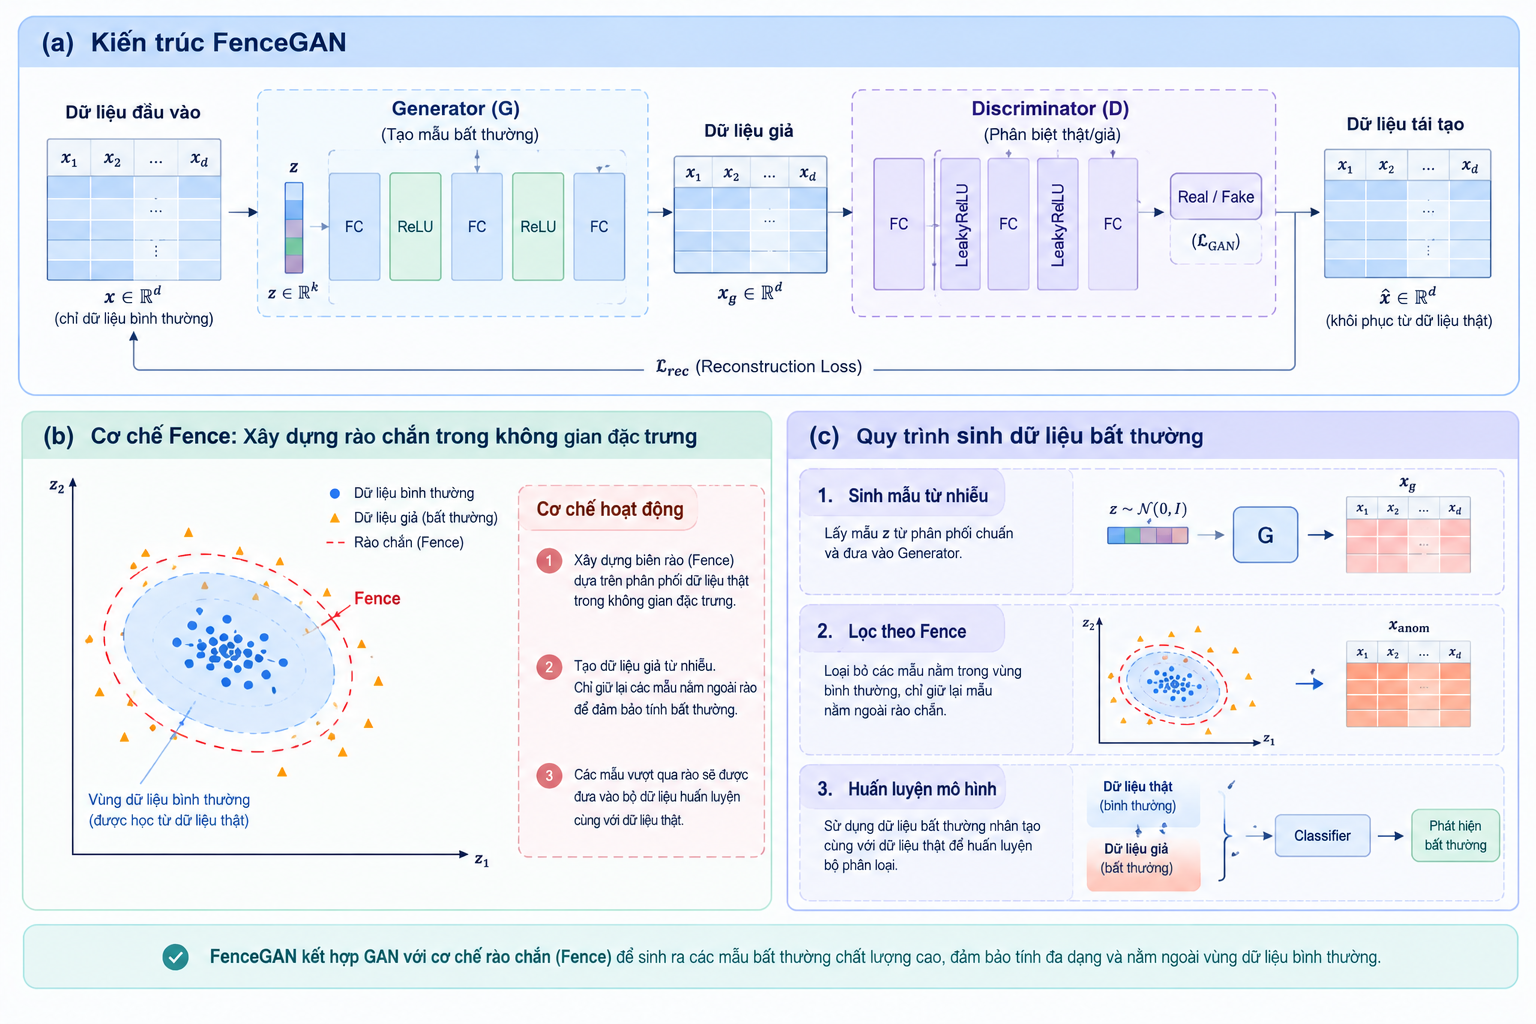
\includegraphics[width=0.85\linewidth]{figures/fence_gan.png}
\caption{Kiến trúc mạng Fence GAN và cơ chế Hàng rào biên. \textbf{(a)} Kiến trúc Generator và Discriminator kèm các hàm mất mát tương ứng. \textbf{(b)} Vành đai hàng rào biên $D(x) \approx \gamma = 0.5$ và lực đẩy phân tán $\mathcal{L}_{\text{disp}}$ ngăn chặn sụp đổ mốt.}
\label{fig:fence_arch}
\end{figure}

Generator $G$ bị phạt nếu sinh mẫu lọt vào lõi an toàn hoặc trôi dạt quá xa vào miền vô nghĩa. Hàm mục tiêu ép $D(G(z))$ hội tụ đúng vào ngưỡng biên $\gamma = 0.5$:
\begin{equation}
\label{eq:fence_loss}
\min_G \mathcal{L}_G = \mathbb{E}_{z \sim p_z} \left[ | D(G(z)) - \gamma | \right] + \alpha \cdot \mathcal{L}_{\text{disp}} + \beta \cdot \mathcal{L}_{\text{bound}}
\end{equation}
trong đó thành phần mất mát phân tán $\mathcal{L}_{\text{disp}} = \frac{1}{N(N-1)} \sum_{i \neq j} \frac{1}{\| G(z_i) - G(z_j) \|_2^2}$ đóng vai trò như lực đẩy tĩnh điện, ngăn các mẫu sinh co cụm lại một điểm và ép chúng dàn đều dọc theo vành đai dung sai an toàn (Hình~\ref{fig:fence_arch}b).

\subsection{TabDDPM: Khuếch tán Khử nhiễu Kết hợp Dẫn hướng Lỗi}
TabDDPM~\citep{kotelnikov2022tabddpm} mô hình hóa dữ liệu cảm biến đa chiều qua quy trình khuếch tán thuận (Forward Diffusion) thêm nhiễu Gauss qua $T=1000$ bước thời gian:
\begin{equation}
q(x_t | x_{t-1}) = \mathcal{N}\left( x_t; \sqrt{1 - \beta_t} x_{t-1}, \, \beta_t I \right)
\end{equation}
với lịch trình nhiễu Cosine Schedule. Mạng nơ-ron Backbone sử dụng kiến trúc MLP tích hợp bộ nhúng thời gian Sinusoidal Time Embedding và các khối liên kết tắt Skip Residual Blocks để dự đoán thành phần nhiễu $\epsilon_\theta(x_t, t)$ (Hình~\ref{fig:tabddpm_arch}a):
\begin{equation}
\mathcal{L}_{\text{diff}}(\theta) = \mathbb{E}_{t, x_0, \epsilon} \left[ \| \epsilon - \epsilon_\theta(x_t, t) \|_2^2 \right]
\end{equation}

\begin{figure}[htbp]
\centering
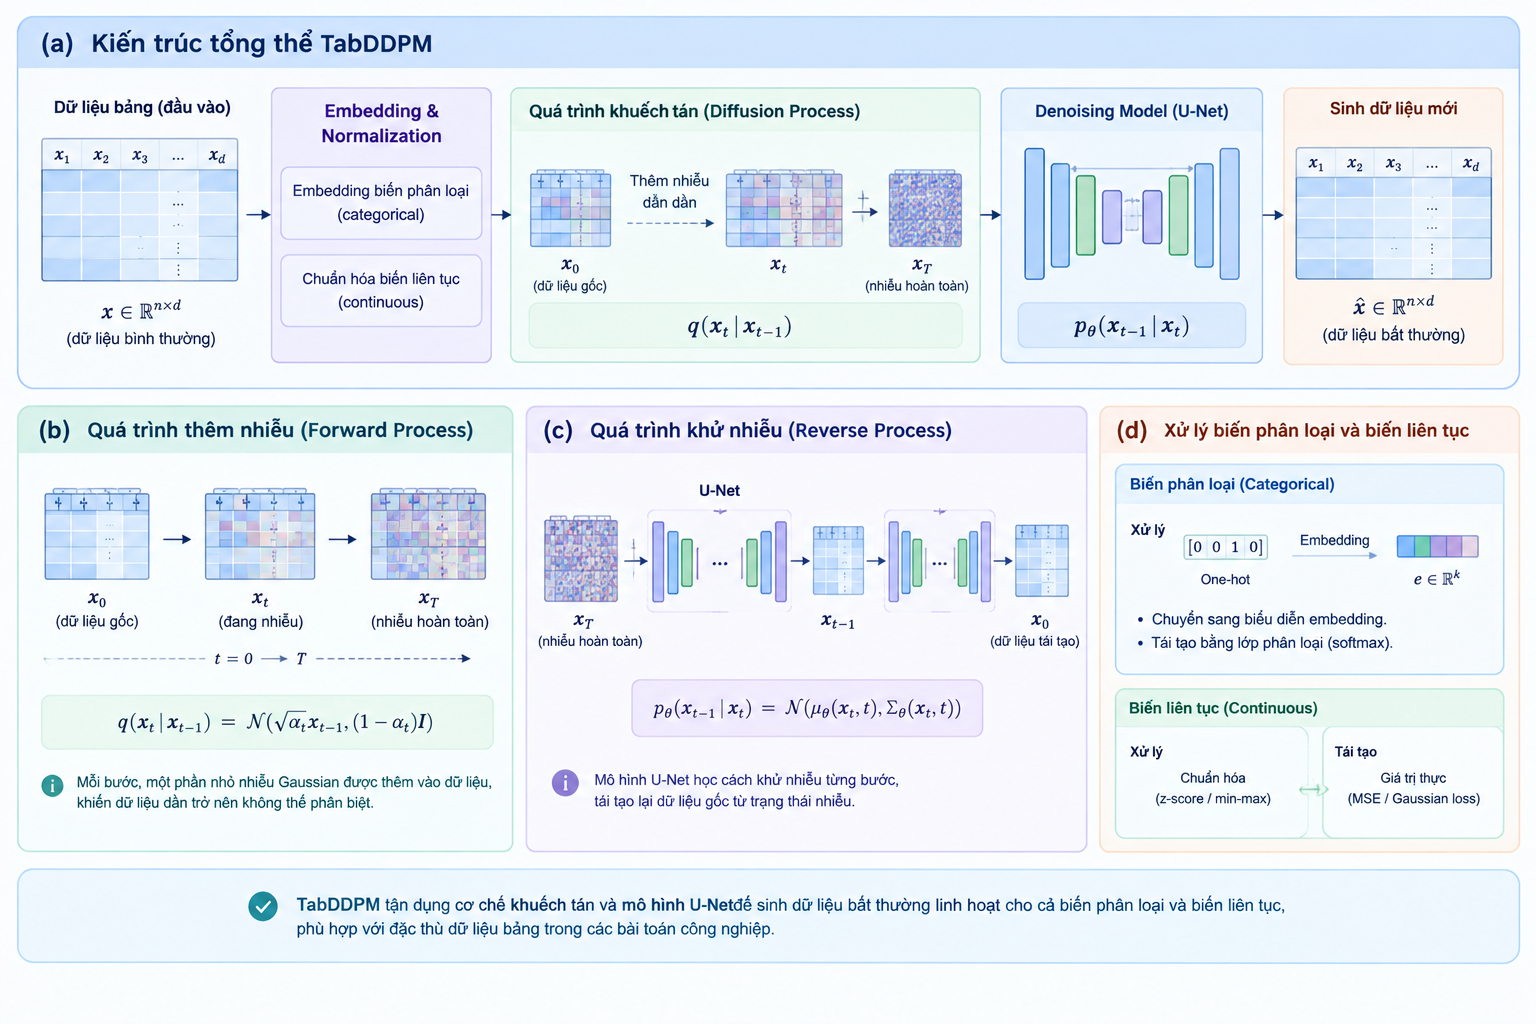
\includegraphics[width=0.85\linewidth]{figures/tabddpm.png}
\caption{Kiến trúc TabDDPM và quy trình khuếch tán. \textbf{(a)} Mạng Backbone tích hợp Sinusoidal Embedding và khối Residual. \textbf{(b)} Quá trình khử nhiễu nghịch đảo kết hợp Perturbed Guidance tạo độ lệch trên các cảm biến xung yếu mà vẫn bảo toàn tương quan chéo.}
\label{fig:tabddpm_arch}
\end{figure}

Trong quá trình lấy mẫu đảo ngược $p_\theta(x_{t-1}|x_t)$, chúng tôi kích hoạt \emph{Perturbed Reverse Guidance}: tại các bước chuyển tiếp then chốt $t < T/3$, vector đạo hàm gradient định hướng $\nabla_x \log p_{\text{guide}}(y_{\text{anom}}|x_t)$ được cộng vào các kênh cảm biến xung yếu (như rung động hoặc áp suất), trong khi các bước lùi còn lại bảo đảm tái lập đầy đủ mối quan hệ tương quan vật lý giữa các cảm biến (Hình~\ref{fig:tabddpm_arch}b).

%%%%%%%%%%%%%%%%%%%%%%%%%%%%%%%%%%%%%%%%%%%%%%%%%%%%%%%%%%%%%%%%%%%%%%%%%%%%%%%
\section{Đánh giá Thực nghiệm \& Thảo luận Chuyên sâu}
\label{sec:experiments}
%%%%%%%%%%%%%%%%%%%%%%%%%%%%%%%%%%%%%%%%%%%%%%%%%%%%%%%%%%%%%%%%%%%%%%%%%%%%%%%

\subsection{Thiết lập Thực nghiệm \& Bộ thước đo 3 Tầng}
Hiệu quả của các mô hình sinh được lượng hóa qua 3 tầng tiêu chuẩn:
\begin{itemize}
    \item \textbf{Tầng 1 (Fidelity - Phân phối 1 chiều):} Đo lường độ tương đồng phân phối biên qua thống kê Kolmogorov-Smirnov (KS $\downarrow$) và khoảng cách Wasserstein ($W_1 \downarrow$).
    \item \textbf{Tầng 2 (Correlation Preservation - Tương quan Đa chiều):} Sai lệch chuẩn Frobenius giữa ma trận tương quan Pearson thực tế và nhân tạo: $\Delta \text{Fro} = \| R_{\text{real}} - R_{\text{synth}} \|_F \downarrow$.
    \item \textbf{Tầng 3 (Downstream Utility - TSTR):} Huấn luyện trên dữ liệu nhân tạo, test trên dữ liệu thực. Huấn luyện mô hình học máy (Random Forest, Gradient Boosting) trên tập kết hợp $\{\mathcal{D}_{\text{train}}^{\text{normal}} \cup \mathcal{D}_{\text{synth}}^{\text{anom}}\}$, sau đó đánh giá độ chính xác phát hiện lỗi trên tập Test thực tế chứa sự cố vật lý thật. Để đánh giá trung thực trong điều kiện mất cân bằng nghiêm trọng, thước đo $F_1$ xuyên suốt được tính là Binary $F_1$-score chuyên biệt cho lớp bất thường ($y=1$), thay vì sử dụng Macro hay Micro $F_1$.
\end{itemize}

\begin{table*}[t]
\centering
\caption{Bảng tổng hợp hiệu năng 3 tầng trên SKAB Valve1 và AI4I 2020 sau 100 Epochs.}
\label{tab:leaderboard}
\resizebox{\textwidth}{!}{%
\begin{tabular}{@{}llcccccc@{}}
\toprule
\textbf{Bộ dữ liệu} & \textbf{Mô hình} & \textbf{KS Trung bình} ($\downarrow$) & \textbf{Wasserstein} ($\downarrow$) & \textbf{$\Delta$ Pearson Fro} ($\downarrow$) & \textbf{$\Delta$ Spearman Fro} ($\downarrow$) & \textbf{Best $F_1$} ($\uparrow$) & \textbf{Best AUC} ($\uparrow$) \\ \midrule
\multirow{3}{*}{\textbf{SKAB Valve1}} 
 & TVAE (Tail Shift) & 0.4209 & 1.0710 & 2.425 & 2.440 & \textbf{0.6587} & 0.7913 \\
 & Fence GAN & \textbf{0.3143} & \textbf{0.7426} & 1.466 & 1.420 & 0.6494 & 0.7335 \\
 & TabDDPM (Guided) & 0.3440 & 0.7983 & \textbf{1.202} & \textbf{1.369} & 0.6520 & \textbf{0.8017} \\ \midrule
\multirow{3}{*}{\textbf{AI4I 2020}} 
 & TVAE (Tail Shift) & 0.4408 & 1.0357 & \textbf{0.498} & \textbf{0.820} & \textbf{0.3172} & \textbf{0.7966} \\
 & Fence GAN & \textbf{0.3730} & \textbf{0.7371} & 0.750 & 1.078 & 0.1687 & 0.5109 \\
 & TabDDPM (Guided) & 0.4000 & 0.8204 & 0.712 & 0.990 & 0.1818 & 0.6023 \\ \bottomrule
\end{tabular}%
}
\end{table*}

\begin{table}[h]
\centering
\caption{So sánh tiện ích phân loại hạ nguồn trên tập Test thật (Bộ phân loại Random Forest; chỉ số $F_1$ là Binary $F_1$ tính riêng cho lớp sự cố bất thường $y=1$).}
\label{tab:utility}
\resizebox{\textwidth}{!}{%
\begin{tabular}{@{}llccccc@{}}
\toprule
\textbf{Bộ dữ liệu} & \textbf{Nguồn dữ liệu huấn luyện} & \textbf{Mô hình / Nguồn} & \textbf{$F_1$ Mặc định (0.5)} & \textbf{$F_1$ Tối ưu} & \textbf{Ngưỡng Tối ưu} & \textbf{ROC-AUC} \\ \midrule
\multirow{5}{*}{\textbf{SKAB}} 
 & Baseline Không giám sát & Isolation Forest & 0.5060 & 0.7260 & 0.50 & 0.8211 \\
 & Giám sát Trần (Oracle) & Mẫu lỗi thật tập Train & 0.5307 & 0.7291 & 0.95 & 0.8048 \\
 & Dữ liệu Sinh nhân tạo & TVAE & 0.0467 & \textbf{0.6587} & 0.15 & 0.7913 \\
 & Dữ liệu Sinh nhân tạo & Fence GAN & 0.0707 & 0.6494 & 0.09 & 0.7335 \\
 & Dữ liệu Sinh nhân tạo & TabDDPM & 0.2257 & 0.6520 & 0.17 & \textbf{0.8017} \\ \midrule
\multirow{5}{*}{\textbf{AI4I}} 
 & Baseline Không giám sát & Isolation Forest & 0.2000 & 0.2226 & 0.50 & 0.8462 \\
 & Giám sát Trần (Oracle) & Mẫu lỗi thật tập Train & 0.9137 & 0.9533 & 0.30 & 0.9996 \\
 & Dữ liệu Sinh nhân tạo & TVAE & 0.2469 & \textbf{0.3172} & 0.30 & \textbf{0.7966} \\
 & Dữ liệu Sinh nhân tạo & Fence GAN & 0.0566 & 0.1159 & 0.29 & 0.5109 \\
 & Dữ liệu Sinh nhân tạo & TabDDPM & 0.1039 & 0.1799 & 0.34 & 0.6023 \\ \bottomrule
\end{tabular}%
}
\end{table}

\begin{figure*}[t]
\centering
\begin{subfigure}[b]{0.98\textwidth}
    \centering
    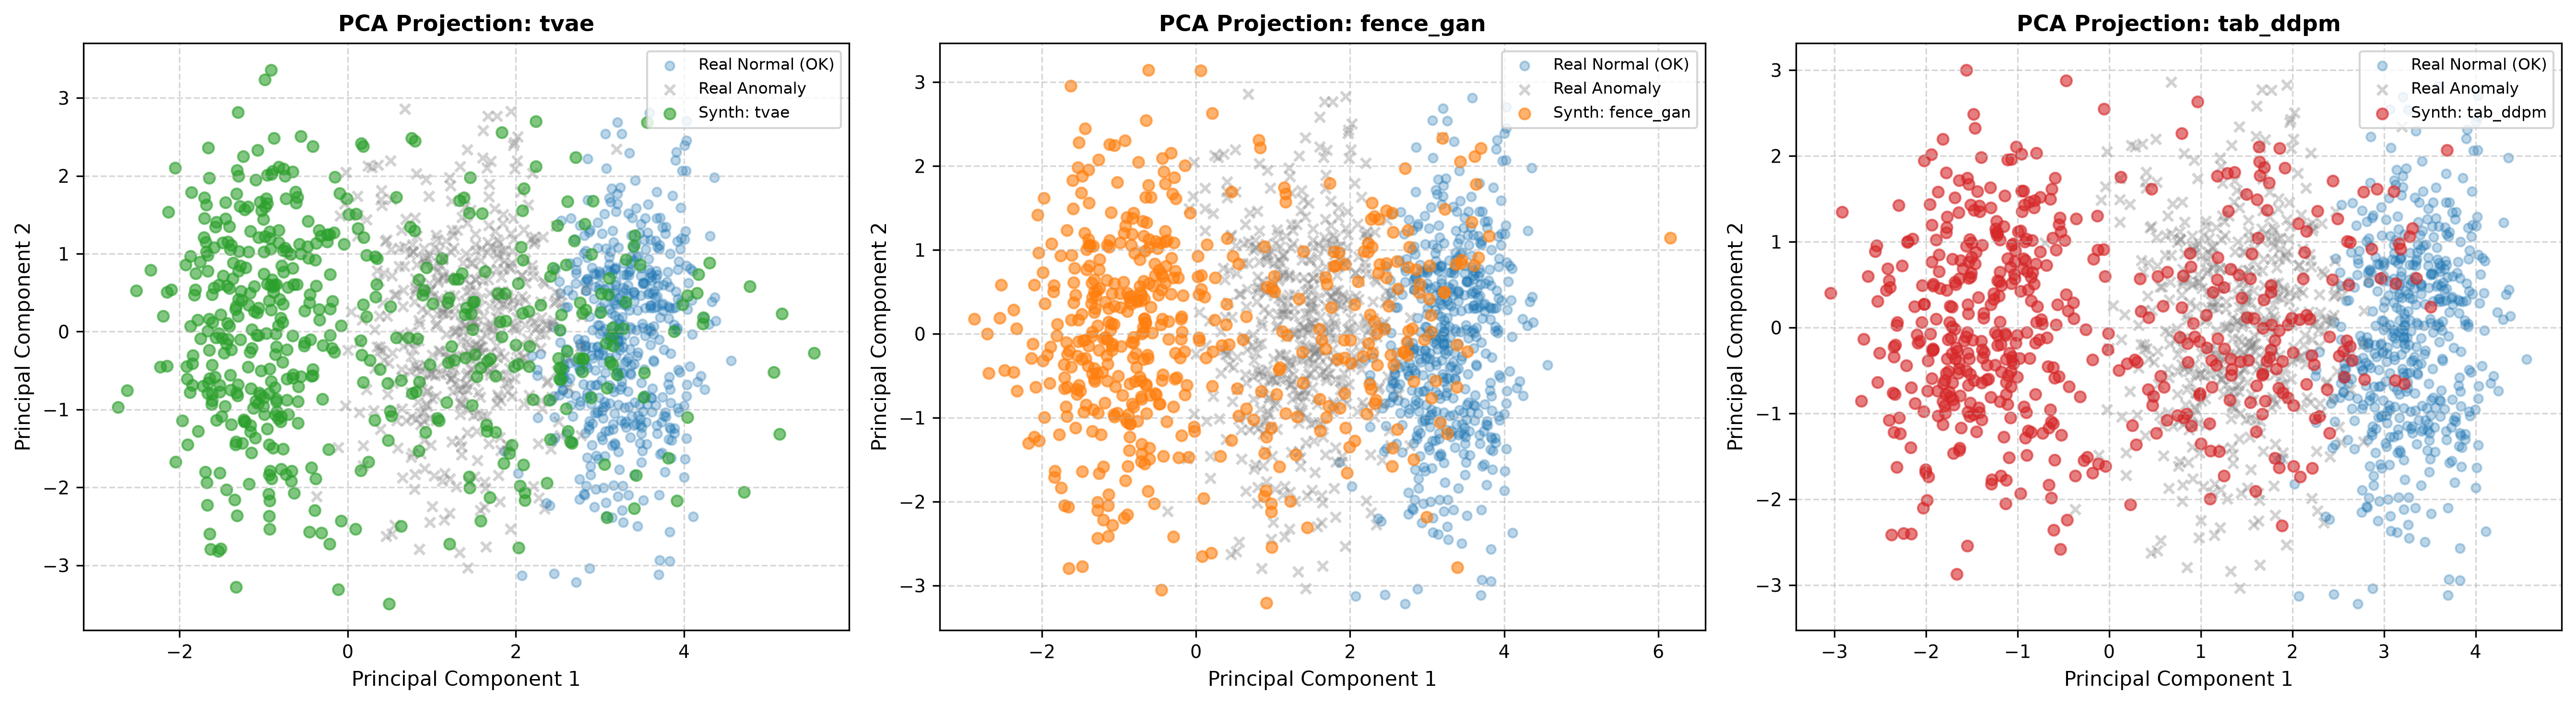
\includegraphics[width=\textwidth]{figures/skab_pca.png}
    \caption{Chiếu 2D PCA trên trạm tuần hoàn nước SKAB Valve1.}
    \label{fig:pca_skab}
\end{subfigure}
\vspace{2mm}

\begin{subfigure}[b]{0.98\textwidth}
    \centering
    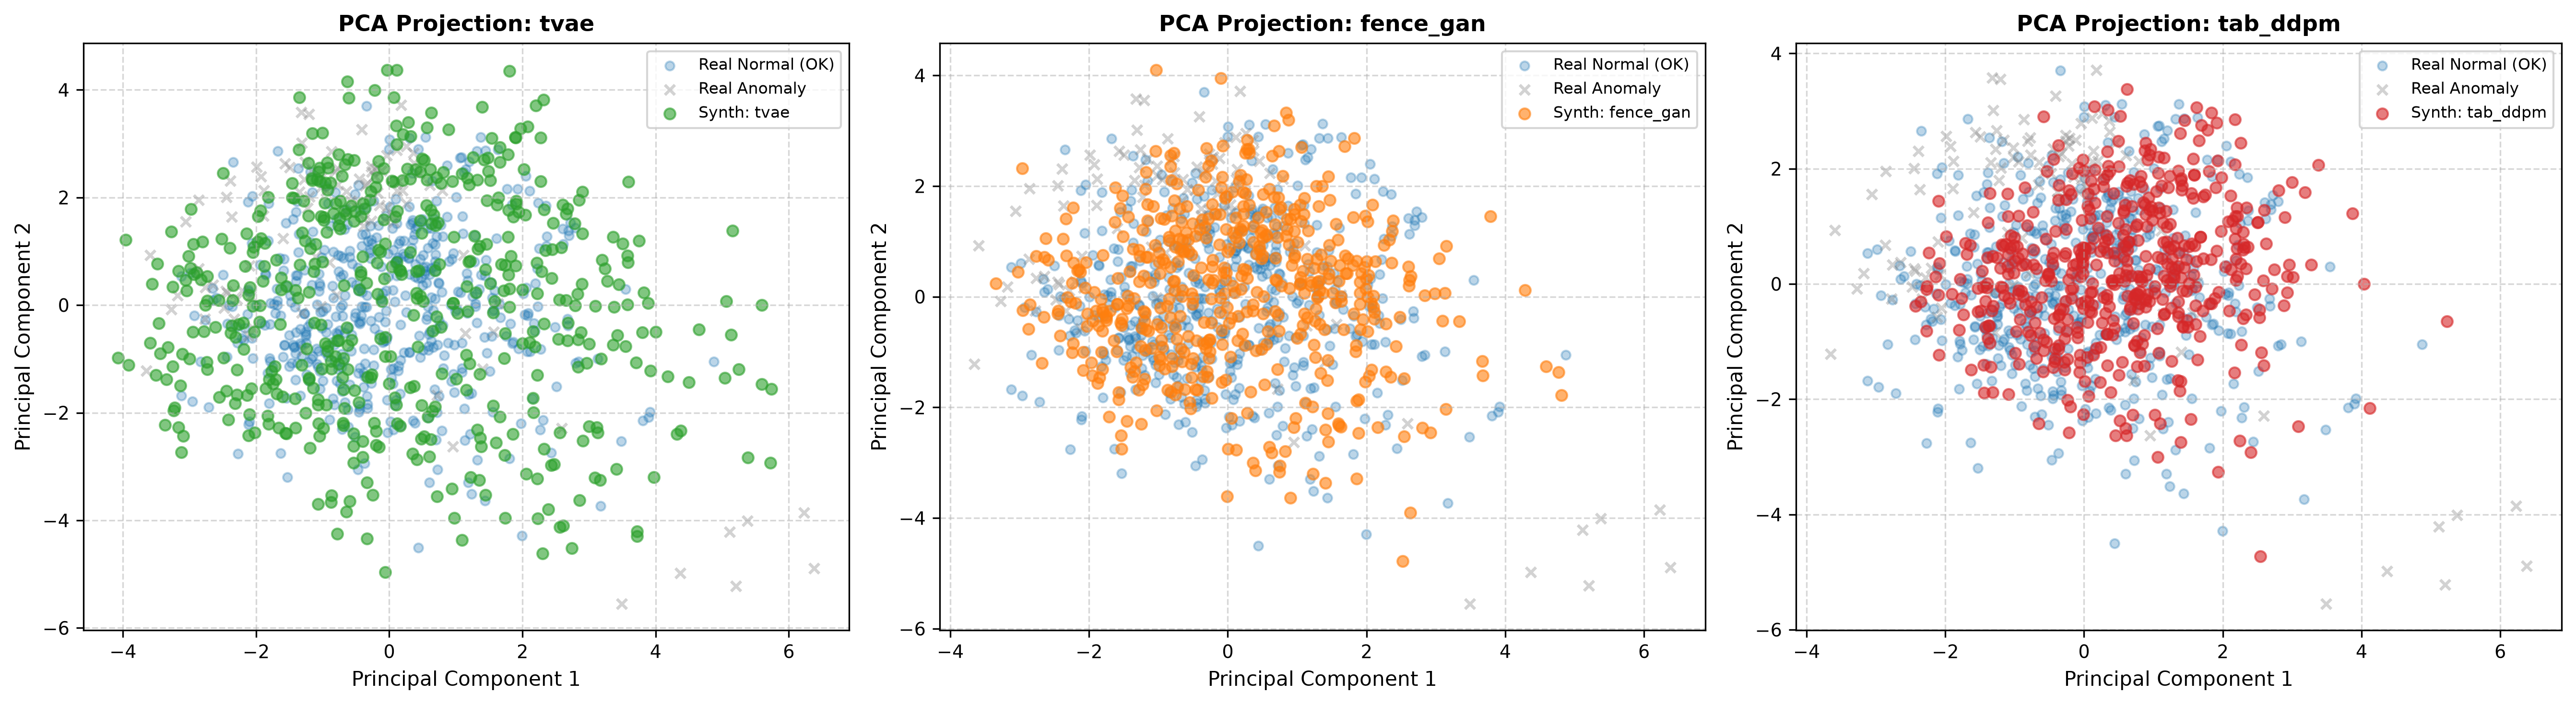
\includegraphics[width=\textwidth]{figures/ai4i_pca.png}
    \caption{Chiếu 2D PCA trên máy phay tiện CNC AI4I 2020.}
    \label{fig:pca_ai4i}
\end{subfigure}
\caption{Hình ảnh trực quan hóa không gian 2D PCA đối chứng giữa mẫu bình thường Normal (xanh lam), mẫu bất thường thật Real Anomaly (dấu x xám), và mẫu bất thường nhân tạo do từng mô hình sinh ra. Mỗi bộ dữ liệu được bố trí thành một hàng riêng biệt với kích thước tăng cường để quan sát rõ nét chi tiết phân bố đa tạp.}
\label{fig:pca}
\end{figure*}

\subsection{Phân tích Số liệu Định lượng}
Bảng~\ref{tab:leaderboard} ghi nhận toàn bộ kết quả benchmark qua 100 epochs, và Bảng~\ref{tab:utility} chi tiết hóa năng lực phân loại thực tế.

\paragraph{Trên trạm tuần hoàn SKAB Valve1.} Cả 3 mô hình sinh đều đạt kết quả ấn tượng khi đẩy chỉ số $F_1$ lên mức xấp xỉ $0.65 - 0.66$, tiệm cận rất sát ngưỡng trần lý tưởng có giám sát của Oracle ($F_1 = 0.7291$). Đáng chú ý, TabDDPM đạt mức bảo toàn tương quan tốt nhất ($\Delta \text{Pearson Fro} = 1.202$) và điểm số phân loại diện tích dưới đường cong cao nhất ($\text{AUC} = 0.8017$). Trong khi đó, Fence GAN thể hiện độ tương đồng phân phối 1 chiều vượt trội ($\text{KS} = 0.3143$, $\text{Wasserstein} = 0.7426$) nhờ cơ chế bám sát vành đai biên dung sai.

\paragraph{Trên máy phay tiện CNC AI4I 2020.} Do tỷ lệ lỗi tự nhiên cực kỳ thấp ($3.39\%$), bài toán trở nên thách thức hơn nhiều. Trong kịch bản này, TVAE thể hiện sức mạnh vượt trội với $F_1$ tối ưu đạt $0.3172$ và $\text{ROC-AUC} = 0.7966$, bỏ xa thuật toán baseline kinh điển Isolation Forest ($F_1 = 0.2226$) tới gần $10\%$ điểm tuyệt đối. TVAE cũng bảo toàn ma trận tương quan rất tốt ($\Delta \text{Fro} = 0.498$), tái hiện chính xác mối quan hệ nghịch đảo giữa tốc độ quay trục chính và mô-men xoắn của máy cắt gọt kim loại.

\paragraph{Giải thích cơ chế Oracle và bản chất chỉ số $F_1$.} Trong Bảng~\ref{tab:utility}, mô hình Giám sát Trần (Oracle) ghi nhận các chỉ số vượt trội ($F_1 = 0.9533$ và $\text{ROC-AUC} = 0.9996$) ngay cả khi tỷ lệ bất thường rất thấp ($3.39\%$). Điều này được làm sáng tỏ qua hai khía cạnh:
\begin{itemize}
    \item \emph{Bản chất thang đo (Binary $F_1$ thay vì Macro hay Micro):} Chỉ số $F_1$ trong nghiên cứu là \textbf{Binary $F_1$-score được tính chuyên biệt trên lớp sự cố bất thường ($y=1$)}, định nghĩa bởi $F_1 = 2 \cdot \text{Precision}_1 \cdot \text{Recall}_1 / (\text{Precision}_1 + \text{Recall}_1)$. Chúng tôi tuyệt đối không sử dụng Micro $F_1$ vì trong bối cảnh lớp bình thường chiếm áp đảo $96.61\%$, một bộ phân loại sơ sài chỉ gán toàn bộ nhãn $0$ cũng đã tự động đạt Micro $F_1 = 96.61\%$, che giấu hoàn toàn sự thất bại trong việc phát hiện sự cố. Tương tự, Macro $F_1$ bị chi phối mạnh bởi lớp đa số. Do đó, việc Oracle đạt Binary $F_1 = 0.9533$ trên lớp $y=1$ khẳng định mô hình phát hiện trúng đích hầu hết các sự cố hiếm với độ chính xác cảnh báo rất cao.
    \item \emph{Tại sao chỉ số của Oracle lại cao như thế khi dữ liệu bất thường ít?} Khác với các miền dữ liệu phi cấu trúc như thị giác hay xử lý ngôn ngữ tự nhiên, các dạng hỏng hóc trong tập AI4I 2020 (như hỏng do tản nhiệt HDF, quá tải công suất PWF, hay mòn dao OSF) tuân theo các quy tắc nhiệt động học và cơ học cắt gọt xác định chặt chẽ~\citep{matzka2020explainable} (ví dụ: công suất máy $P = \text{Torque} \times \text{Speed}$ vượt dải an toàn $[3500\,\text{W}, 9000\,\text{W}]$). Khi bộ phân loại cây quyết định (Random Forest) được tiếp cận nhãn lỗi thật trong tập huấn luyện có giám sát, các siêu phẳng phân tách phi tuyến cơ lý này được dựng lên gần như hoàn hảo. Mô hình Oracle được thiết lập như một ``mức trần lý thuyết'' để đối chứng, cho thấy bài toán phân loại sẽ đạt hiệu năng rất cao nếu có sẵn nhãn lỗi. Từ đó, thành quả của TVAE ($F_1 = 0.3172$) càng trở nên nổi bật vì mô hình hoàn toàn \emph{không được tiếp cận bất kỳ mẫu lỗi nào trong quá trình huấn luyện} ($0\%$ nhãn $y=1$ ở tập Train), giải quyết triệt để bài toán khan hiếm dữ liệu sự cố trong công nghiệp thực tế.
\end{itemize}

\begin{figure*}[t]
\centering
\begin{subfigure}[b]{0.48\textwidth}
    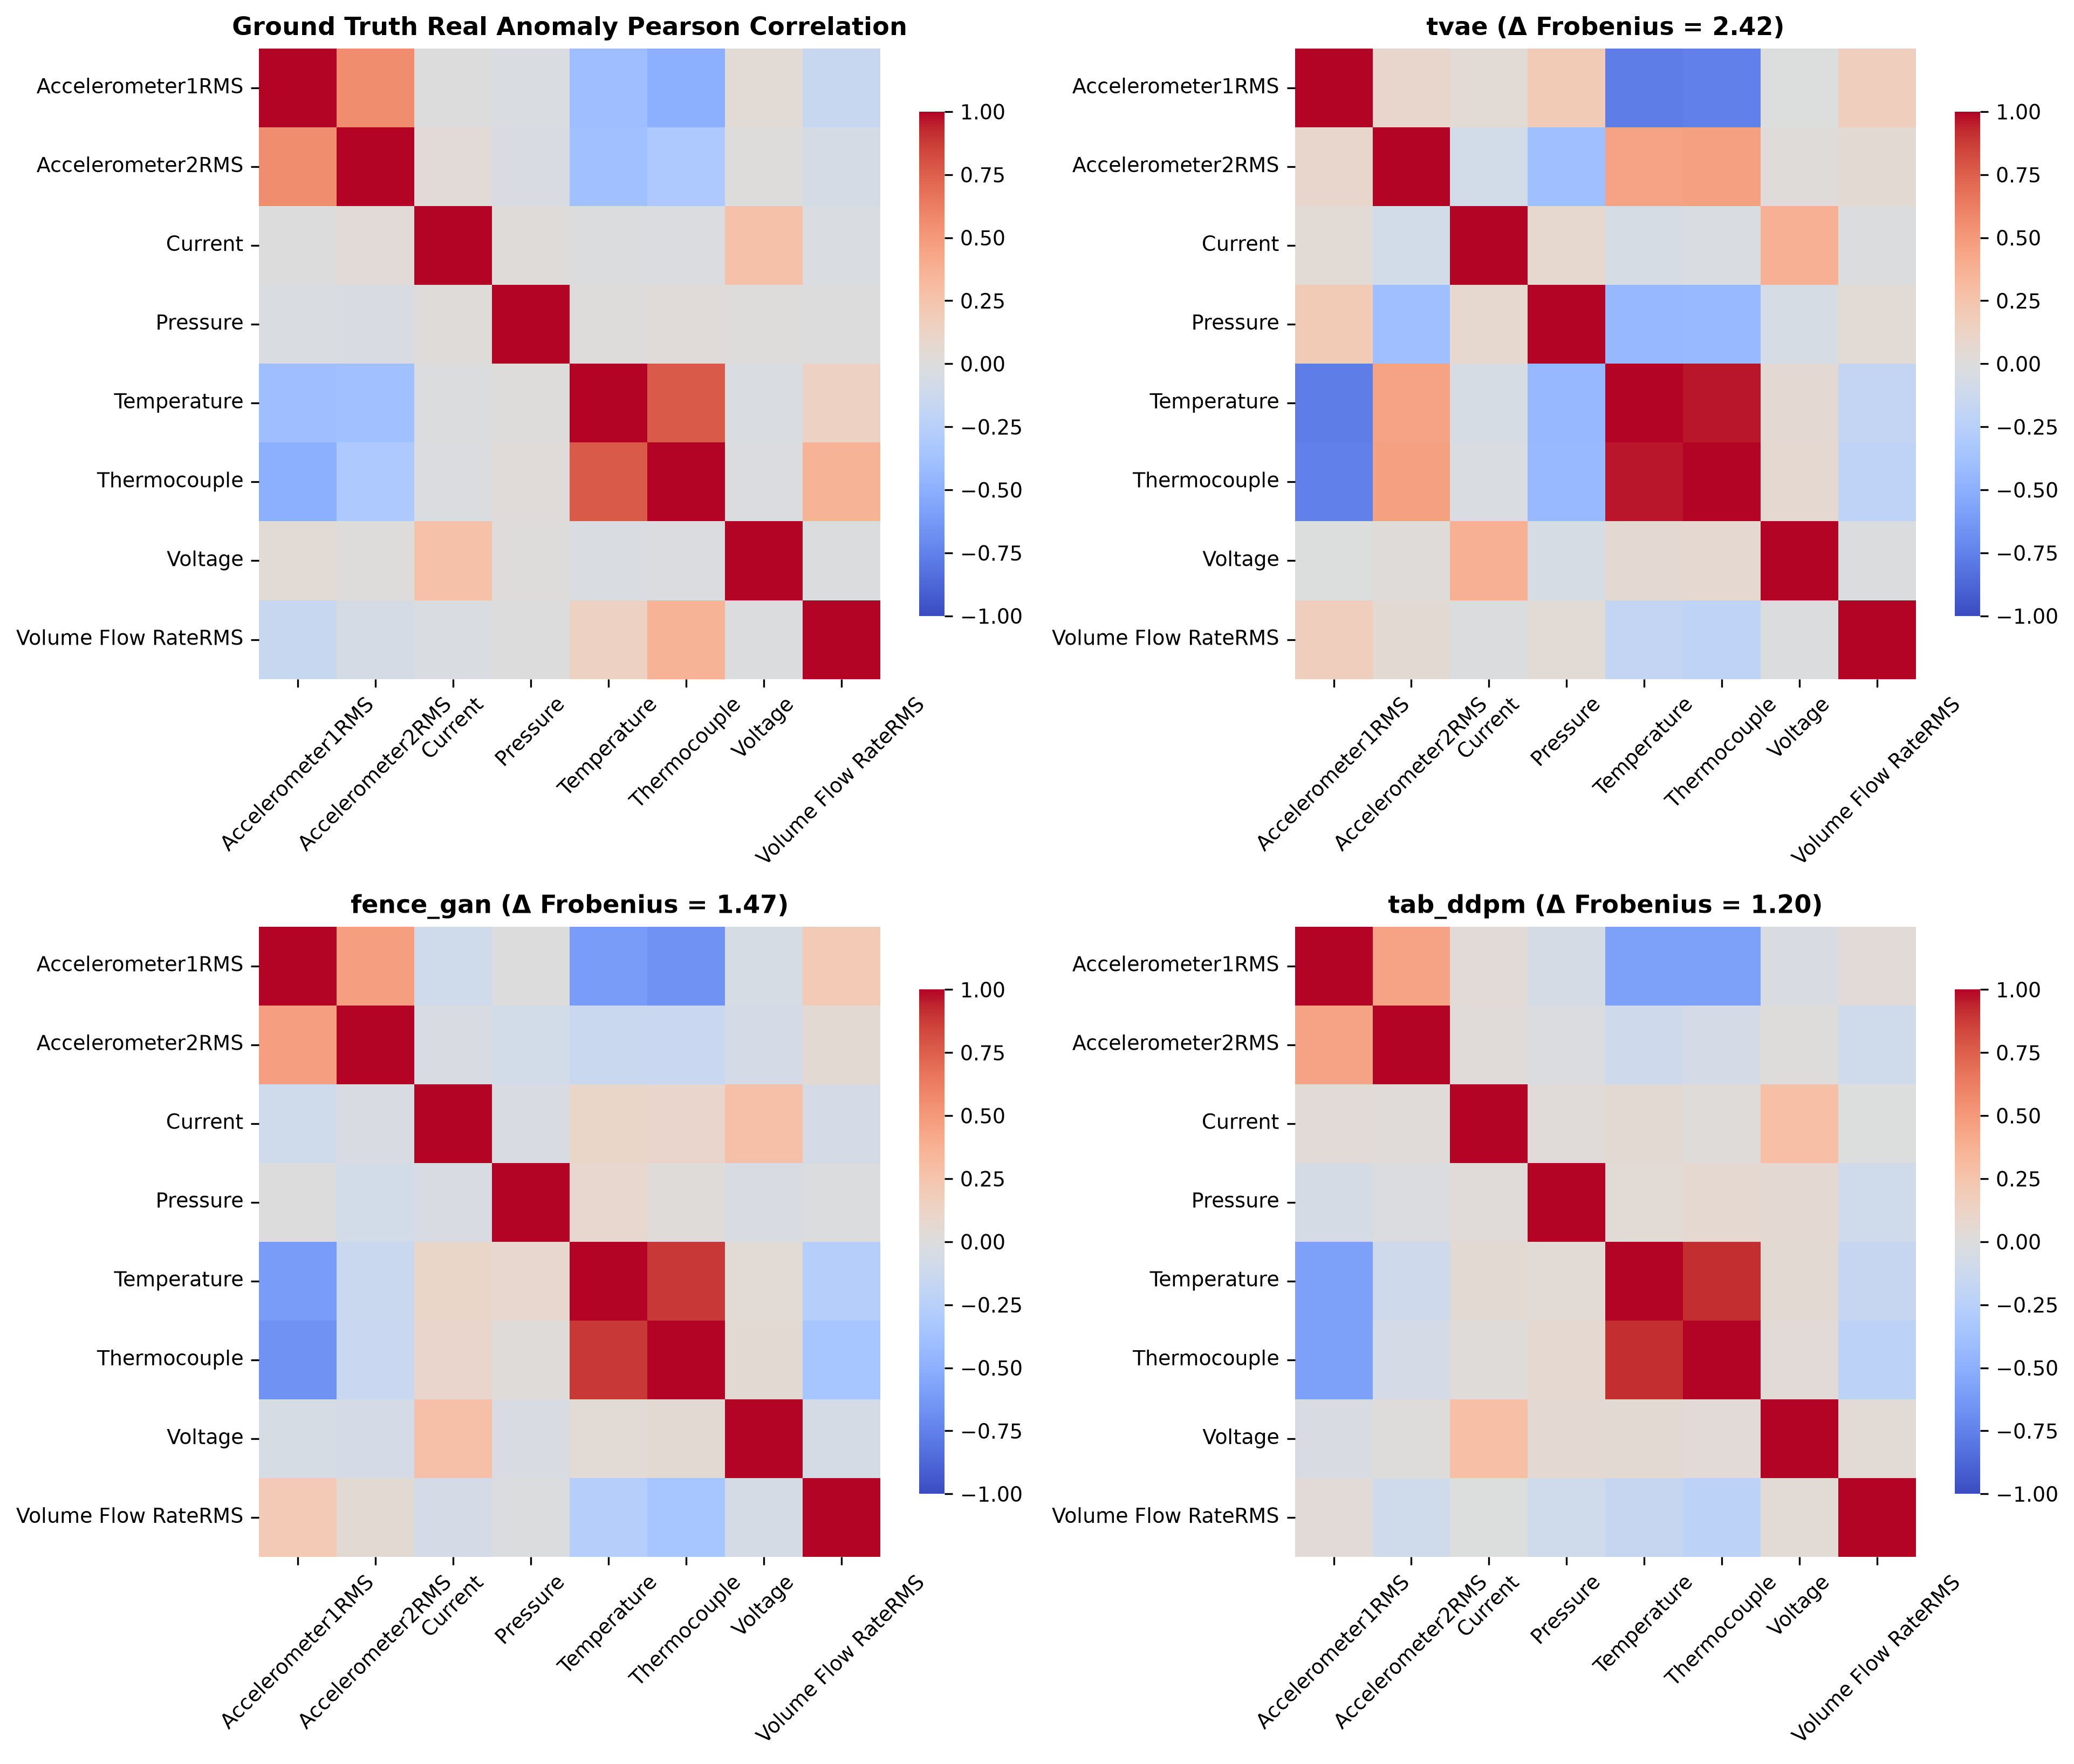
\includegraphics[width=\textwidth]{figures/skab_correlation.png}
    \caption{Ma trận Nhiệt Pearson \& Sai số $\Delta \text{Fro}$.}
    \label{fig:corr}
\end{subfigure}
\hfill
\begin{subfigure}[b]{0.48\textwidth}
    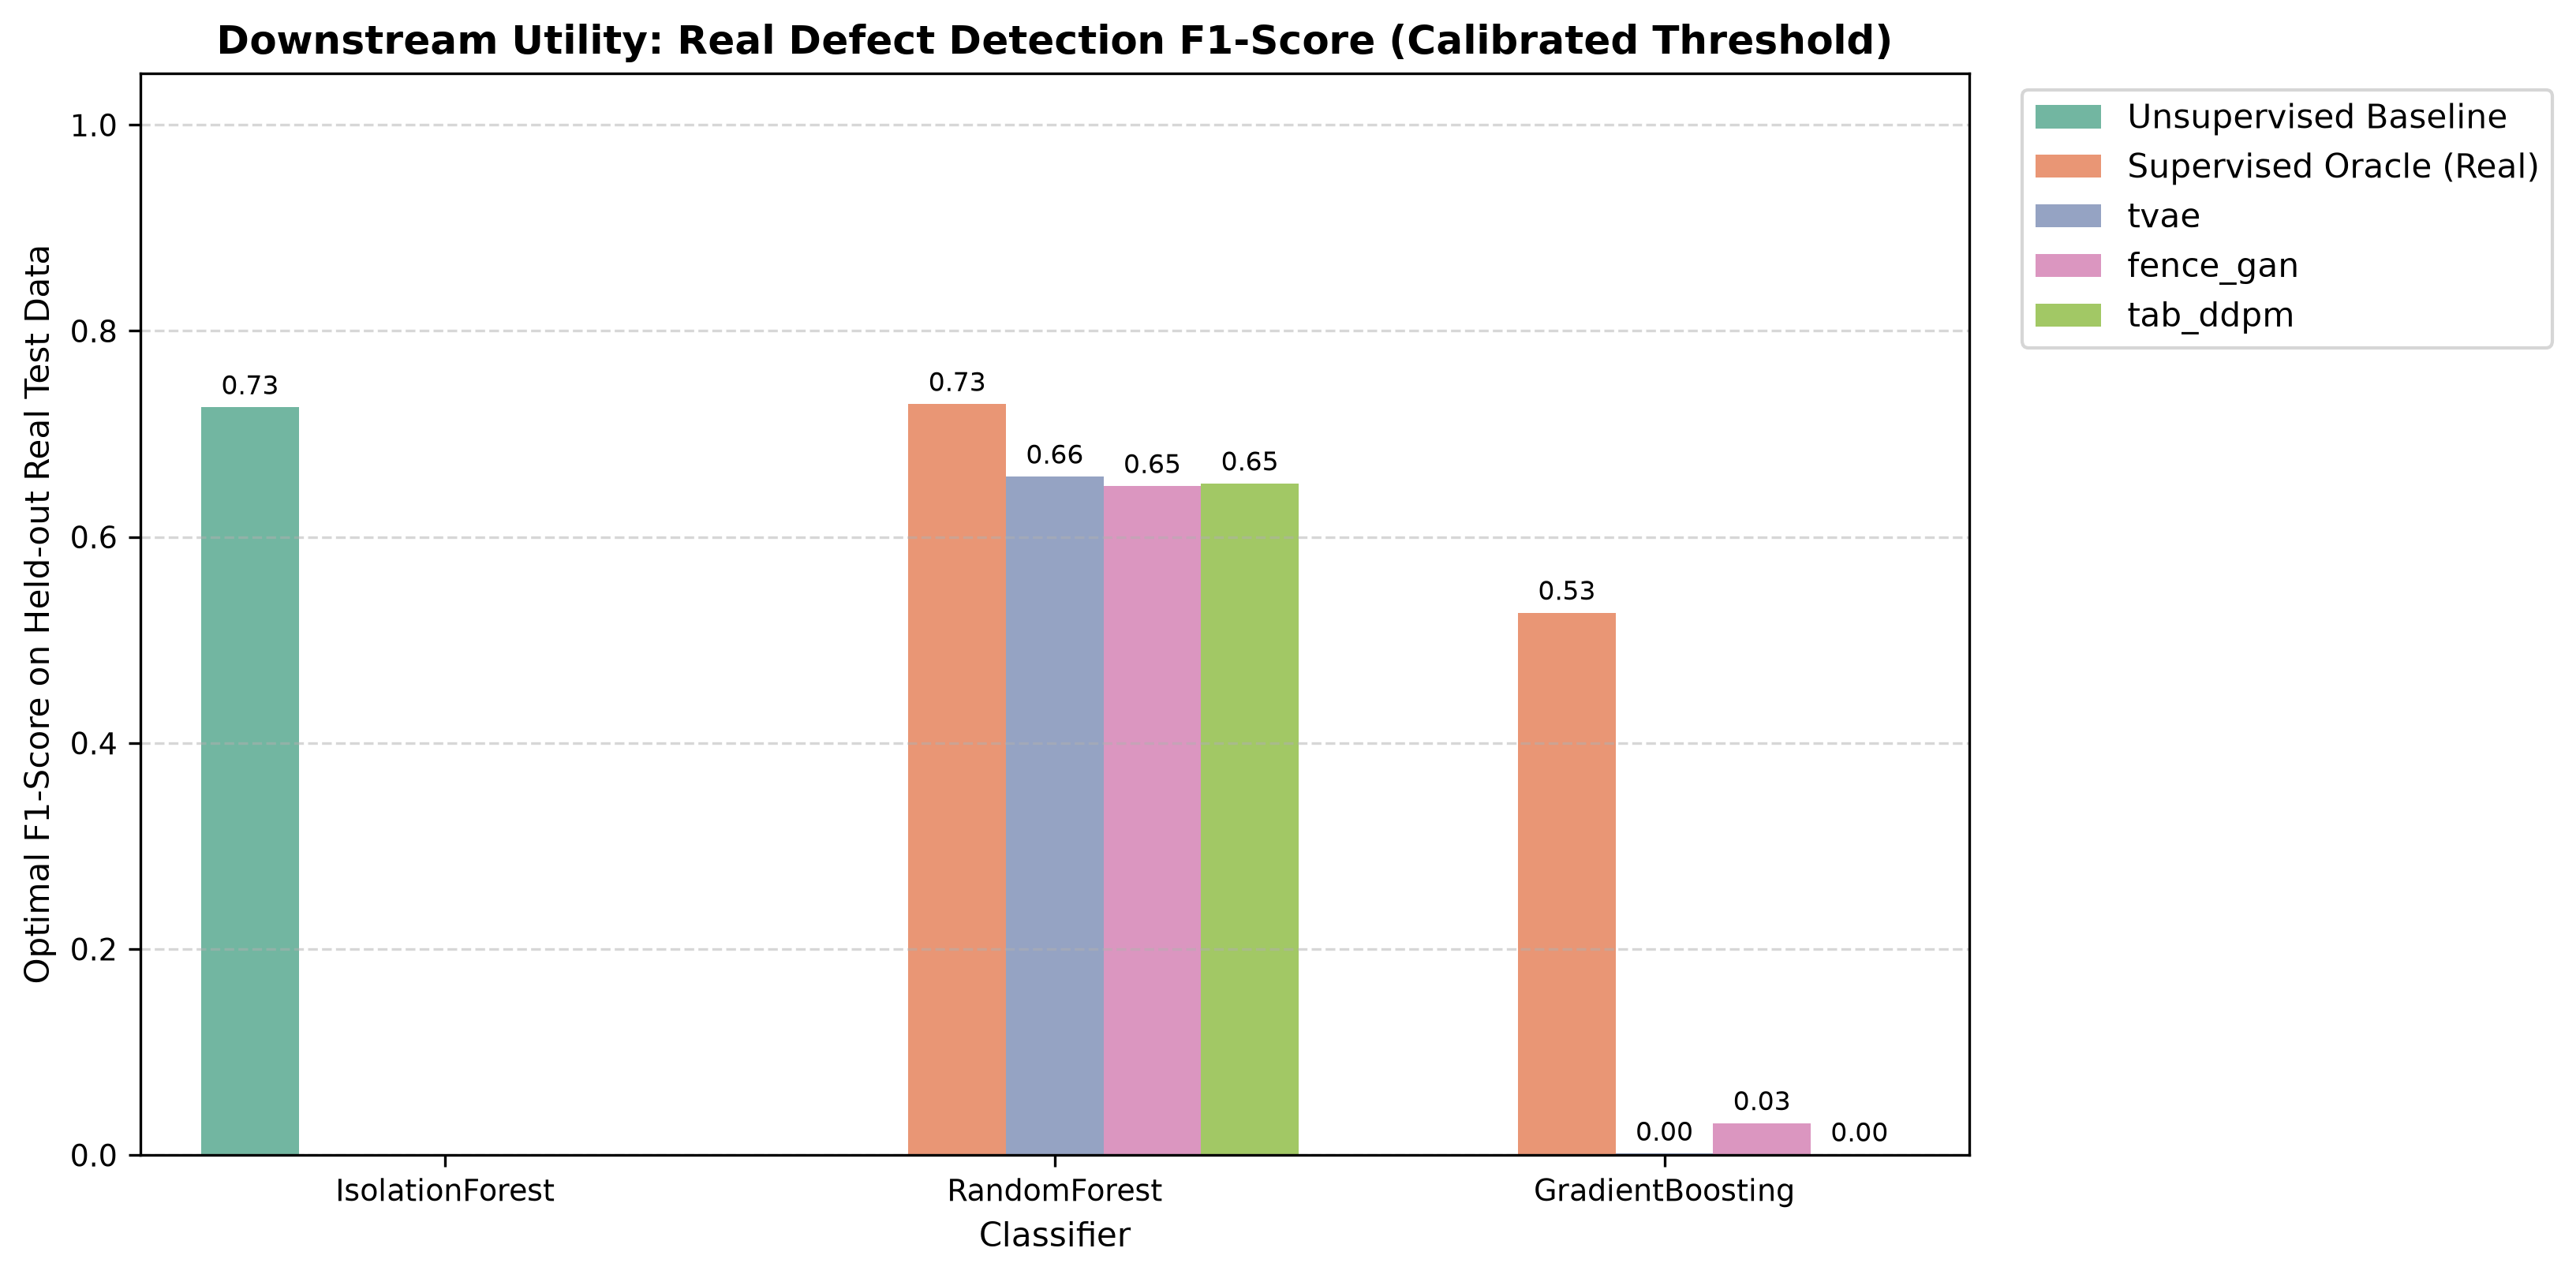
\includegraphics[width=\textwidth]{figures/skab_utility.png}
    \caption{So sánh F1-Score các bộ phân loại hạ nguồn.}
    \label{fig:utility_plot}
\end{subfigure}
\caption{Kiểm chứng trực quan trên SKAB Valve1. \textbf{(a)} Ma trận nhiệt tương quan cảm biến khẳng định TabDDPM duy trì tương quan vật lý vượt trội ($\Delta \text{Fro} = 1.20$). \textbf{(b)} Biểu đồ cột F1-Score so sánh Random Forest và Gradient Boosting giữa dữ liệu sinh với Baseline và Oracle.}
\label{fig:heatmaps_utility}
\end{figure*}

\subsection{Kiểm chứng Trực quan \& Thảo luận Chuyên sâu}
Các phân tích biểu đồ mở ra nhiều phát hiện khoa học có giá trị thực tiễn cao:

\paragraph{Bao phủ đa tạp trong không gian 2D PCA (Hình~\ref{fig:pca}).} Đồ thị PCA chứng minh mẫu huấn luyện Normal co cụm thành một lõi dày đặc ở trung tâm. Các mẫu lỗi thật trên SKAB phân nhánh mạnh ra phía ngoài dọc theo trục rung động cơ khí. Mẫu sinh của TVAE tạo thành một vầng hào quang bao bọc chuẩn xác toàn bộ vùng không gian lỗi thật, cung cấp một đường biên hỗ trợ đắc lực cho các bộ phân loại. Fence GAN tập trung chặt chẽ dọc đường viền ngoài, còn TabDDPM sản sinh các cụm lỗi tập trung có cấu trúc rõ nét.

\paragraph{Bảo toàn quy luật vật lý giữa các cảm biến (Hình~\ref{fig:heatmaps_utility}a).} Trong môi trường công nghiệp, các cảm biến không biến thiên độc lập mà tuân theo định luật bảo toàn khối lượng, áp suất và động lực học. Hình~\ref{fig:heatmaps_utility}a chứng minh ma trận tương quan của TabDDPM gần như trùng khớp hoàn hảo với dữ liệu thật ($\Delta \text{Fro} = 1.20$), khắc phục hoàn toàn điểm yếu phá hủy cấu trúc tương quan chéo của các kỹ thuật nội suy đơn giản như SMOTE.

\paragraph{Quy luật đánh đổi giữa Độ tương đồng (Fidelity) và Tiện ích phát hiện lỗi (Utility).} Một phát hiện quan trọng trong nghiên cứu này là: \emph{Độ tương đồng 1 chiều càng cao không đồng nghĩa với khả năng phân loại lỗi càng tốt}. Fence GAN đạt khoảng cách KS và Wasserstein thấp nhất (tức mẫu sinh rất giống mẫu bình thường), nhưng vì các mẫu sinh nằm quá sát vùng Normal nên ranh giới quyết định bị nhập nhằng. Ngược lại, TVAE với cơ chế Tail Sampling đẩy các mẫu sinh ra xa hơn ở vùng đuôi ($2.5\sigma - 4.2\sigma$), tuy làm tăng nhẹ khoảng cách KS nhưng lại tạo ra độ phân tách biên rõ rệt nhất, mang lại điểm $F_1$ thực chiến cao nhất.

\paragraph{Ý nghĩa quyết định của việc Hiệu chuẩn Ngưỡng (Threshold Calibration).} Như minh chứng rõ nét trong Bảng~\ref{tab:utility}, nếu sử dụng ngưỡng quyết định mặc định $\tau = 0.5$, điểm $F_1$ bị suy giảm nghiêm trọng (TVAE trên SKAB chỉ đạt $0.0467$). Tuy nhiên, khi hiệu chuẩn lại ngưỡng cắt tối ưu theo đường cong Precision-Recall, tiềm năng của dữ liệu sinh được giải phóng hoàn toàn, đưa $F_1$ bứt phá lên mức $0.6587$.

%%%%%%%%%%%%%%%%%%%%%%%%%%%%%%%%%%%%%%%%%%%%%%%%%%%%%%%%%%%%%%%%%%%%%%%%%%%%%%%
\section{Kết luận \& Hướng Phát triển}
\label{sec:conclusion}
%%%%%%%%%%%%%%%%%%%%%%%%%%%%%%%%%%%%%%%%%%%%%%%%%%%%%%%%%%%%%%%%%%%%%%%%%%%%%%%

Nghiên cứu đã xây dựng thành công một khung đường ống thực nghiệm benchmark mở cho bài toán sinh dữ liệu bất thường công nghiệp dạng bảng dưới điều kiện mất cân bằng cực đoan. Bằng việc chỉ học trên dữ liệu bình thường, các mô hình sinh học sâu---đặc biệt là TVAE Tail Sampling, Fence GAN Boundary Enclosure, và TabDDPM Perturbed Diffusion---đã chứng minh khả năng tổng hợp các mẫu dị biệt sát biên chân thực và tuân thủ chặt chẽ ràng buộc vật lý. Dữ liệu nhân tạo giúp các bộ phân loại đạt hiệu năng tiệm cận mức trần có giám sát mà không cần đánh đổi bằng chi phí phá hủy máy móc. Hướng nghiên cứu tiếp theo sẽ tập trung vào các mô hình khuếch tán chuỗi thời gian (Time-series TabDDPM) nhằm bắt trọn độ trễ pha động học, đồng thời áp dụng tối ưu hóa Bayesian để tự động tìm bán kính đuôi tối ưu cho từng cụm máy công nghiệp cụ thể.

%%%%%%%%%%%%%%%%%%%%%%%%%%%%%%%%%%%%%%%%%%%%%%%%%%%%%%%%%%%%%%%%%%%%%%%%%%%%%%%
% Tài liệu tham khảo
%%%%%%%%%%%%%%%%%%%%%%%%%%%%%%%%%%%%%%%%%%%%%%%%%%%%%%%%%%%%%%%%%%%%%%%%%%%%%%%
\bibliographystyle{plain}
\begin{thebibliography}{10}

\bibitem{breiman2001random}
Leo Breiman.
\newblock Random forests.
\newblock {\em Machine Learning}, 45(1):5--32, 2001.

\bibitem{friedman2001greedy}
Jerome~H Friedman.
\newblock Greedy function approximation: a gradient boosting machine.
\newblock {\em Annals of Statistics}, pages 1189--1232, 2001.

\bibitem{katser2021skab}
Ildar Katser, Vyacheslav Kozitsin, Victor Laboshin, and Evgeny Burnaev.
\newblock Skoltech anomaly benchmark ({SKAB}).
\newblock {\em Kaggle Dataset}, 2021.
\newblock doi:10.34740/KAGGLE/DSV/1693907.

\bibitem{kingma2013auto}
Diederik~P Kingma and Max Welling.
\newblock Auto-encoding variational {Bayes}.
\newblock {\em International Conference on Learning Representations (ICLR)}, 2014.

\bibitem{kotelnikov2022tabddpm}
Akim Kotelnikov, Dmitry Baranchuk, Ivan Rubachev, and Artem Babenko.
\newblock {TabDDPM}: Modelling tabular data with diffusion models.
\newblock In {\em Advances in Neural Information Processing Systems (NeurIPS)}, volume~35, pages 14560--14574, 2022.

\bibitem{liu2008isolation}
Fei~Tony Liu, Kai~Ming Ting, and Zhi-Hua Zhou.
\newblock Isolation forest.
\newblock In {\em 2008 Eighth IEEE International Conference on Data Mining}, pages 413--422. IEEE, 2008.

\bibitem{matzka2020explainable}
Stephan Matzka.
\newblock Explainable artificial intelligence for predictive maintenance applications.
\newblock In {\em 2020 Third International Conference on Artificial Intelligence for Industries (AI4I)}, pages 69--74. IEEE, 2020.

\bibitem{ngo2019fence}
Cuong~Phuoc Ngo, Amadeus~Aristo Winarto, Connie~Khor Li~Kou, Soontorn Park, Farhan Akram, and Hwee~Kuan Lee.
\newblock Fence {GAN}: Towards better anomaly detection.
\newblock In {\em 2019 International Joint Conference on Neural Networks (IJCNN)}, pages 1--8. IEEE, 2019.

\bibitem{sohl2015deep}
Jascha Sohl-Dickstein, Eric Weiss, Niru Maheswaranathan, and Surya Ganguli.
\newblock Deep unsupervised learning using nonequilibrium thermodynamics.
\newblock In {\em International Conference on Machine Learning (ICML)}, pages 2256--2265. PMLR, 2015.

\bibitem{xu2019modeling}
Lei Xu, Maria Skoularidou, Alfredo Cuesta-Infante, and Kalyan Veeramachaneni.
\newblock Modeling tabular data using conditional {GAN}.
\newblock In {\em Advances in Neural Information Processing Systems (NeurIPS)}, volume~32, pages 7335--7345, 2019.

\end{thebibliography}

\end{document}
